\chapter{Energy Conservation in Maxwell’s Wheel}

Date: 8/11/2020

\section{Aim}

The aim of this experiment is to understand the principle of conservation of energy and how it is distributed among the translational and rotational motion. We study the combination of rotational and transalational motion in a Maxwell's wheel




\section{Background Theory}

In transalational motion of an object, the entire object can be considered as a single point. All points of the object move in similar fashion and hence can be described from the same equation  of motion.  
However, rotational objects cannot be replaced by a single point as it is done in transalational motion.
Different points on the object are moving with different  speeds, depending on the distance from the axis of rotation. \\
The potential energy of the Maxwell's wheel is given by the expression,
\begin{equation}
    U =  mgh
\end{equation}
where m is the mass of the object and h is the maximum height . \\
The transalational kinetic energy of the Maxwell's wheel is given by the expression,
\begin{equation}
    KE =  \frac{1}{2}mv^2
\end{equation}
where m is the mass of the object and  v is the linear speed.\\
The rotational kinetic energy of the Maxwell's wheel is given by the expression,
\begin{equation}
    RE =  \frac{1}{2}I\omega^2
\end{equation}
where I is the moment of the Inertia and  $\omega$ is the angular speed.\\
As the wheel rotates, the change in the potential is equal to the sum of the transalational kinetic and rotational kinetic energy.
\begin{equation}
    \Delta U = KE + RE
\end{equation}
\begin{equation}
    mg\Delta h = \frac{1}{2}mv^2  + \frac{1}{2}I\omega^2
\end{equation}
where  $\Delta h$ is the height of the Maxwell's wheel from the surface of the table. \\
We can write $v = \omega r$, giving us the equation. 
\begin{equation}
    mg\Delta h = \frac{1}{2}mv^2  + \frac{1} { 2 r ^2}I v ^  2
\end{equation}
Re-arranging equation 7.6 and making $v^2$ as the subject gives us the following equation.
\begin{equation}
    v^2 = \frac{2mgr^2}{mr^2 + I} \Delta h
\end{equation}
\newpage
\section{Description of Setup}
\begin{figure}[h!]
    \centering
    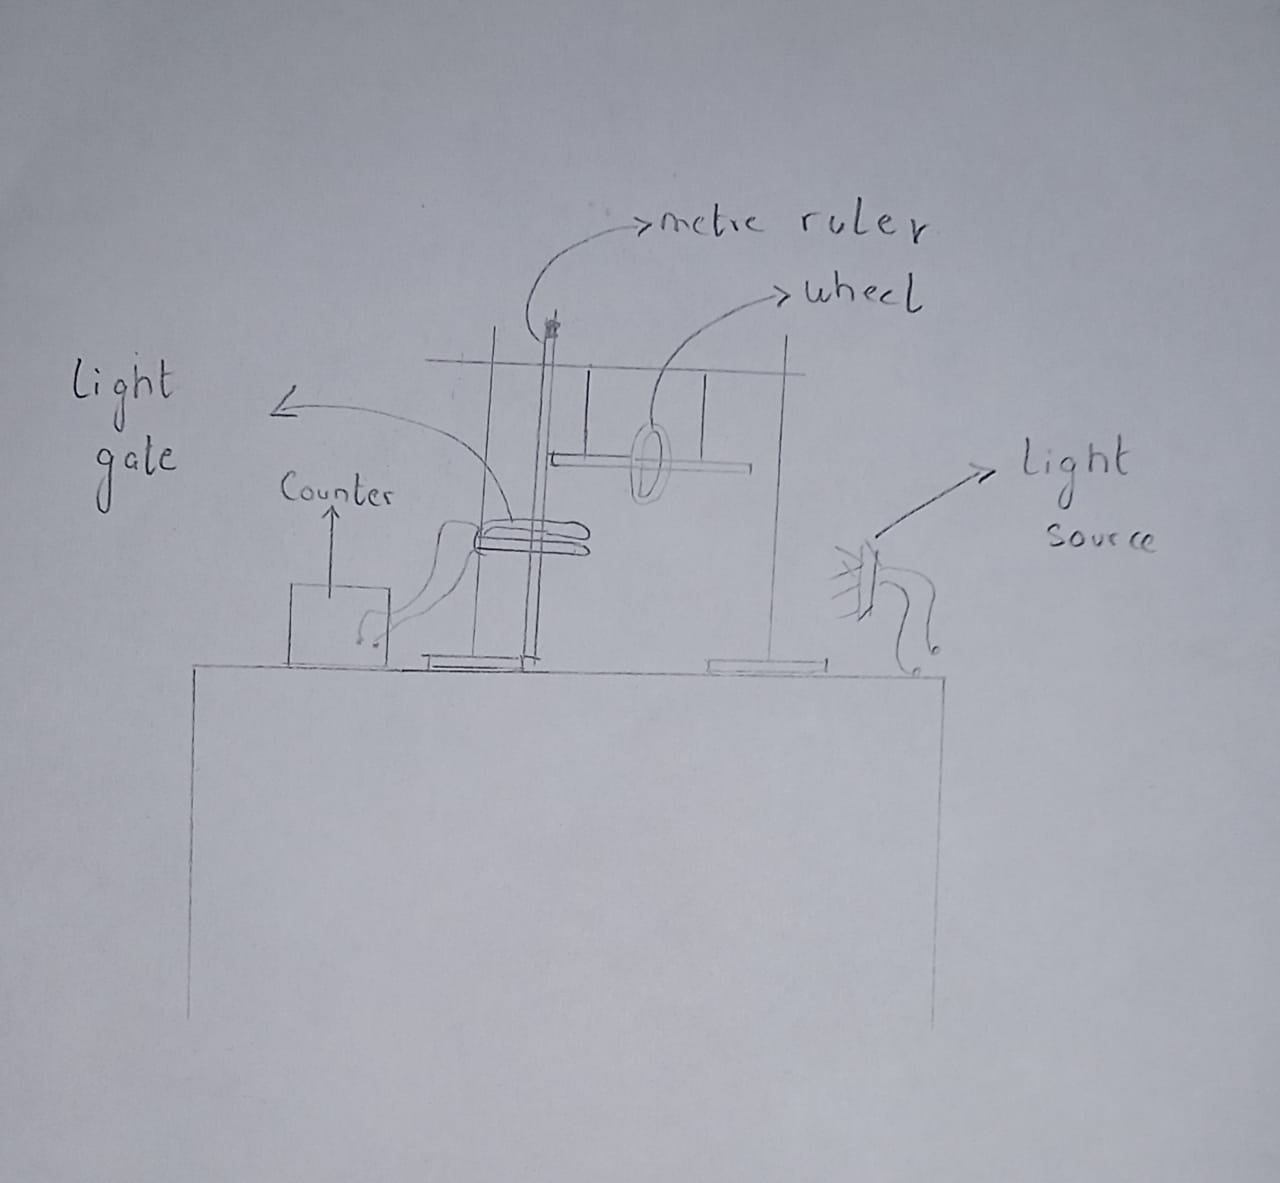
\includegraphics[width=\textwidth]{figures/Sktech.jpeg}
    \caption{Sketch of the experiment setup.}
    \label{fig:yx}
\end{figure}
Here the Light Gate and counter is used to measure translation speed v at given heights, the metre scale is used to measure the height of the Maxwell wheel $\Delta h$ with respect from the surface of the table.
\section{Method / Procedure}
The Maxwell's wheel is rotated up about its spindle such that the cord uniformly wounds about the spindle. When the wheel is released, it then falls as the chord unwinds. The speed of the translational of the wheel is calculated using the formula $ v = \frac{d}{t}$ where d is the diameter of the spindle and t is the time recorded by the counter. The height $\Delta h$ is adjusted by changing the position of the light gate. The above process is repeated 5 times for each $\Delta h$ and we chose 5 different values of the $\Delta h$.  The graph of $v^2$ vs $\Delta h$ and then slope of best fit is determined. The value of the best slope and the equation 7.7 is used to calculate the value of the moment of Inertia, I
\section{Data}
The type B uncertainty associated with the height h is $0.002m$ and the time is $0.0000003s$.  The mass of the object is $ m = 0.450 kg $ , the diameter of the wheel is  $ 0.13m$ and the diameter of the spindle is $ 0.003 m$

\begin{center}
\begin{tabular}{|l|l|l|l|l|}
\hline
\multicolumn{1}{|c|}{s.No} & \multicolumn{1}{c|}{$\Delta h(m)$} & \multicolumn{1}{c|}{Avg t(s)} & \multicolumn{1}{c|}{v (m/s)} & \multicolumn{1}{c|}{ $v^2 (m^2/s^2) $}\\ \hline
1                          & 0.44                                            & 0.0321104                     & 0.186855                     & 0.034914921                                                                           \\ \hline
2                          & 0.37                                            & 0.03222875                    & 0.186169                     & 0.034658964                                                                           \\ \hline
3                          & 0.3                                             & 0.032023333                   & 0.187363                     & 0.035105036                                                                           \\ \hline
4                          & 0.23                                            & 0.031566                      & 0.190078                     & 0.03612962                                                                            \\ \hline
5                          & 0.16                                            & 0.031749                      & 0.188982                     & 0.035714321                                                                           \\ \hline
\end{tabular}
\end{center}

\section{Data Analysis}

\begin{center}
\begin{adjustbox}{width=1\textwidth}
\begin{tabular}{|l|l|l|l|l|l|l|l|}
\hline
s.NO & TypeTimeA    & TypeBTime & TimeUncertainity & TimeVelocity    & HeightB     & TimeHeight      & Combined        \\ \hline
1    & 0.000324683  & 0.0000003 & 0.000325         & 0.0000001360356 & 0.000204124 & 0.0000156804345 & 0.0000156810245 \\ \hline
2    & 0.0000350323 & 0.0000003 & 0.000035         & 0.0000000128247 & 0.000204124 & 0.0000156804345 & 0.0000156804397 \\ \hline
3    & 0.0001901485 & 0.0000003 & 0.000190         & 0.0000000555547 & 0.000204124 & 0.0000156804345 & 0.0000156805329 \\ \hline
4    & 0.0001874448 & 0.0000003 & 0.000187         & 0.0000000417399 & 0.000204124 & 0.0000156804345 & 0.0000156804900 \\ \hline
5    & 0.0001901485 & 0.0000003 & 0.000190         & 0.0000000252239 & 0.000204124 & 0.0000156804345 & 0.0000156804548 \\ \hline
\end{tabular}
\end{adjustbox}
\end{center}

\begin{figure}[h!]
    \centering
    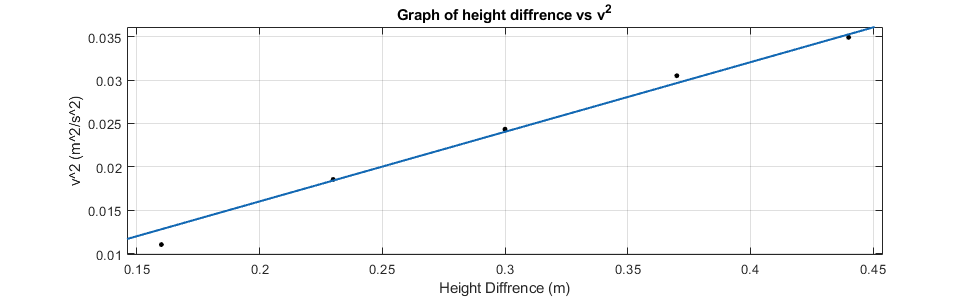
\includegraphics[width=\textwidth]{figures/AvgH_v2.png}
    \caption{Graph of y vs x}
    \label{fig:yx}
\end{figure}
\begin{equation}
    v^2 = 0.0814 \Delta h
\end{equation}
The gradient $ a = 0.0814 $

\begin{equation}
    gradient = \frac{2mgr^2}{mr^2 + I}  \Delta h
\end{equation}
Making the I,moment of inertia as a subject gives us the equation
\begin{equation}
    I  = \frac{2mgr^2 -amr^2}{a}
\end{equation}
where a is the gradient, m is the mass of object, g is the gravitational acceleration and r is the radius of the spindle. 
\begin{itemize}
    \item $ m = 0.450 kg $
    \item $ g = 9.80665 m/s^2 $
    \item $ r = 0.003 m$
\end{itemize}
Using the equation 7.8 and the above values we can calculate the value of I, the moment of Inertia 
$$ I  = \frac{2 \times 0.450 \times 9.80664 \times 0.003^2 -0.0814 \times 0.450 \times 0.003^2}{0.0814} = 0.97178 \times 10^{-3} kg m^2$$

\begin{figure}[h!]
    \centering
    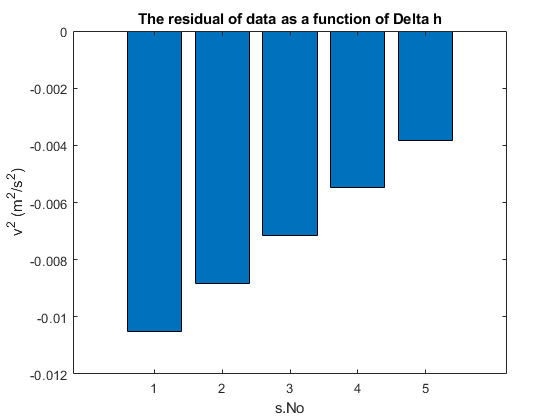
\includegraphics[width=\textwidth]{figures/residual_h.png}
    \caption{Residual of actual as a function of delta H}
    \label{fig:yx}
\end{figure}



\section{Discussion \& Conclusion}

The graph of $v^2$ vs $\Delta h$ is a linear which suggests a linear trend. Furthermore, the actual value of the Moment of Inertia I, $1.03 \times 10^-3 kg m^2$ is very close to the measured value of the Moment of Inertia, $0.9718 \times 10^-3 kg m^2 $ . The residual plot of the actual data as the function of $\Delta h$  shows a certain pattern which indicates the pattern of a systematic error. One of the possible sources of these systematic errors energy losses due to friction


\section{MATLAB Script}
\lstinputlisting{matlabCodes/Experiment7.m}



